\documentclass[../main.tex]{subfiles}
\begin{document}
%=========================================TRUYỆN CHÍNH========================================
\subsection*{1. Đặt vấn đề bài toán}
\addcontentsline{toc}{subsection}{Đặt vấn đề bài toán}

\textbf{Phát biểu bài toán:} Cho một hình ảnh X bất kỳ, nhiệm vụ là tạo ra một câu mô tả (chú thích) tự động mô tả nội dung của hình ảnh đó một cách chính xác và tự nhiên.

Input:
\begin{itemize}
    \item Một hình ảnh X
\end{itemize}

Output:
\begin{itemize}
    \item Một câu văn bản Y mô tả nội dung của hình ảnh X
\end{itemize}

\subsection*{2. Ý tưởng chung}
\addcontentsline{toc}{subsection}{Ý tưởng chung}

Khi đối diện với một bức ảnh bất kỳ, con người thường dựa vào kinh nghiệm, hiểu biết về thế giới và khả năng nhận diện các đối tượng, hành động, bối cảnh để mô tả nội dung ảnh bằng ngôn ngữ tự nhiên. Ý tưởng của bài toán này là mô phỏng quá trình đó bằng cách kết hợp sức mạnh của mô hình học sâu đa phương thức (CLIP) để trích xuất đặc trưng hình ảnh và mô hình sinh ngôn ngữ (LSTM) để tạo ra câu chú thích phù hợp.

Cụ thể, hệ thống sẽ sử dụng CLIP để chuyển đổi ảnh thành vector đặc trưng mang thông tin nội dung, sau đó LSTM sẽ tiếp nhận đặc trưng này và sinh ra câu mô tả tự động. Nhờ đó, mô hình có thể học cách liên kết giữa hình ảnh và ngôn ngữ, từ đó tạo ra các chú thích sát nghĩa, tự nhiên và giàu thông tin cho ảnh đầu vào mà không cần sự can thiệp thủ công của con người.

\subsection*{3. Mô tả bộ dữ liệu sử dụng và tiền xử lí tạo dữ liệu huấn luyện}
\addcontentsline{toc}{subsection}{Mô tả bộ dữ liệu sử dụng và tiền xử lí tạo dữ liệu huấn luyện}

\subsubsection*{3.1 Bộ dữ liệu sử dụng}
\addcontentsline{toc}{subsubsection}{Bộ dữ liệu sử dụng}

\begin{itemize}
    \item Sử dụng bộ dữ liệu Flickr8k
    \item Mỗi ảnh đi kèm nhiều chú thích (caption) do con người viết, mô tả nội dung ảnh.
    \item Dữ liệu gồm hai phần chính:
    \begin{itemize}
        \item Thư mục ảnh: chứa các file ảnh (dataset/Images/)
        \item File chú thích: file văn bản (dataset/captions.txt) với mỗi dòng gồm tên ảnh và chú thích, phân tách bởi dấu phẩy.
    \end{itemize}
\end{itemize}

\subsubsection*{3.2 Tiền xử lý dữ liệu}
\addcontentsline{toc}{subsubsection}{Tiền xử lý dữ liệu}

Việc xử lí dữ liệu gồm các bước sau:
\begin{itemize}
    \item \textbf{Bước 1: } Đọc và gom nhóm chú thích: Đọc file chú thích, gom tất cả caption tương ứng với từng ảnh vào một dictionary
    \item \textbf{Bước 2: } Xây dựng từ điển (Vocabulary)
    \begin{itemize}
        \item Duyệt qua toàn bộ caption, tách từ (tokenize) bằng NLTK.
        \item Đếm tần suất xuất hiện của từng từ.
        \item Chỉ thêm các từ xuất hiện đủ số lần tối thiểu (ví dụ: ≥5) vào từ điển để giảm nhiễu.
        \item Gán chỉ số cho các token đặc biệt: <PAD>, <SOS>, <EOS>, <UNK>.
    \end{itemize}
    \item \textbf{Bước 3: } Mã hóa caption
    \begin{itemize}
        \item Mỗi caption được chuyển thành một chuỗi số nguyên dựa trên từ điển (numericalize).
        \item Thêm token <SOS> ở đầu và <EOS> ở cuối mỗi caption.
    \end{itemize}
    \item \textbf{Bước 4: } Tiền xử lý ảnh
    \begin{itemize}
        \item Ảnh được đọc bằng PIL, chuyển sang RGB.
        \item Ảnh được resize và chuẩn hóa bằng hàm preprocess của CLIP để phù hợp với encoder.
    \end{itemize}
    \item \textbf{Bước 5: } Tạo Dataset và DataLoader
    \begin{itemize}
        \item Mỗi phần tử của dataset gồm:
        \begin{itemize}
            \item Ảnh đã tiền xử lý (tensor)
            \item Caption đã mã hóa (chuỗi số nguyên)
        \end{itemize}
        \item Sử dụng DataLoader để tạo batch, tự động padding caption về cùng độ dài trong batch.
    \end{itemize}
    \item \textbf{Bước 6: } Chia tập dữ liệu: Ngẫu nhiên chia dữ liệu thành 3 phần:
    \begin{itemize}
        \item Tập huấn luyện (train): 80\% dữ liệu
        \item Tập kiểm tra (val): 10\% dữ liệu
        \item Tập kiểm thử (test): 10\% dữ liệu
    \end{itemize}
\end{itemize}

\subsection*{4. Lựa chọn mô hình và hàm chi phí}
\addcontentsline{toc}{subsection}{Lựa chọn mô hình và hàm chi phí}

\subsubsection*{4.1 Mô hình}
\addcontentsline{toc}{subsubsection}{Mô hình}

Trong bài toán tạo chú thích ảnh, nhóm em lựa chọn kiến trúc kết hợp giữa mô hình CLIP và LSTM có tích hợp cơ chế Attention. Cụ thể, đặc trưng hình ảnh được trích xuất từ encoder CLIP (ViT-B/32), sau đó được đưa vào mạng LSTM nhiều lớp để sinh ra chuỗi từ mô tả. Cơ chế Attention giúp mô hình tập trung vào các đặc trưng quan trọng của ảnh tại mỗi bước sinh từ, từ đó nâng cao chất lượng chú thích.

\subsubsection*{4.2 Hàm chi phí}
\addcontentsline{toc}{subsubsection}{Hàm chi phí}
Để huấn luyện mô hình, nhóm em đã sử dụng hàm mất mát Cross-Entropy Loss, vốn là lựa chọn phổ biến cho các bài toán sinh chuỗi. Hàm này đo lường sự khác biệt giữa phân phối xác suất dự đoán của mô hình và nhãn thực tế (chuỗi từ đúng). Ngoài ra, trong quá trình sinh chú thích, nhóm em áp dụng thêm các kỹ thuật như length penalty và repetition penalty để tối ưu hóa chất lượng câu sinh ra, hạn chế lặp từ và khuyến khích độ dài hợp lý.

Công thức hàm mất mát tổng quát như sau:

$$
\mathcal{L} = -\frac{1}{N} \sum_{i=1}^N \sum_{t=1}^{T_i} \log P(y_t^{(i)} \mid y_{1:t-1}^{(i)}, X^{(i)})
$$

Trong đó:
\begin{itemize}
    \item $y_t^{(i)}$ là từ thứ $t$ trong câu mô tả (caption) của ảnh thứ $i$
    \item $y_{1:t-1}^{(i)}$ là dãy từ trước đó
    \item $X^{(i)}$ là đặc trưng hình ảnh đầu vào
    \item $N$ là số lượng mẫu trong một batch huấn luyện.
\end{itemize}

\subsubsection*{4.3 Tham số được sử dụng}
\addcontentsline{toc}{subsubsection}{Tham số được sử dụng}

\begin{itemize}
    \item embed\_size (Kích thước vector embedding cho mỗi từ trong caption) = 256
    \item hidden\_size (Số chiều của trạng thái ẩn (hidden state) trong LSTM) = 512
    \item batch\_size (Số lượng mẫu (ảnh và caption) được xử lý trong mỗi lần lặp (iteration) của quá trình huấn luyện) = 32
    \item learning\_rate (Tốc độ học của thuật toán tối ưu (Adam)) = 3e-4
    \item num\_epochs  (Số vòng huấn luyện) = 15
    \item use\_clip\_cache (Các đặc trưng ảnh từ CLIP sẽ được tính trước và lưu lại để tăng tốc quá trình huấn luyện) = True
    \item early\_stopping\_patience (Số epoch tối đa cho phép mô hình không cải thiện trên tập validation trước khi dừng sớm quá trình huấn luyện) = 2
    \item attention (Bật/tắt cơ chế Attention trong mô hình LSTM) = True
    \item beam\_size (Kích thước beam search khi sinh caption) = 5
\end{itemize}

\subsubsection*{4.4 Kết quả huấn luyện}
\addcontentsline{toc}{subsubsection}{Kết quả huấn luyện}

Quá trình huấn luyện mô hình được thực hiện trong 15 epoch với batch size là 32. Đồ thị dưới đây thể hiện sự thay đổi của giá trị loss trên tập huấn luyện và tập validation qua từng epoch:

\begin{figure}[H]
    \centering
    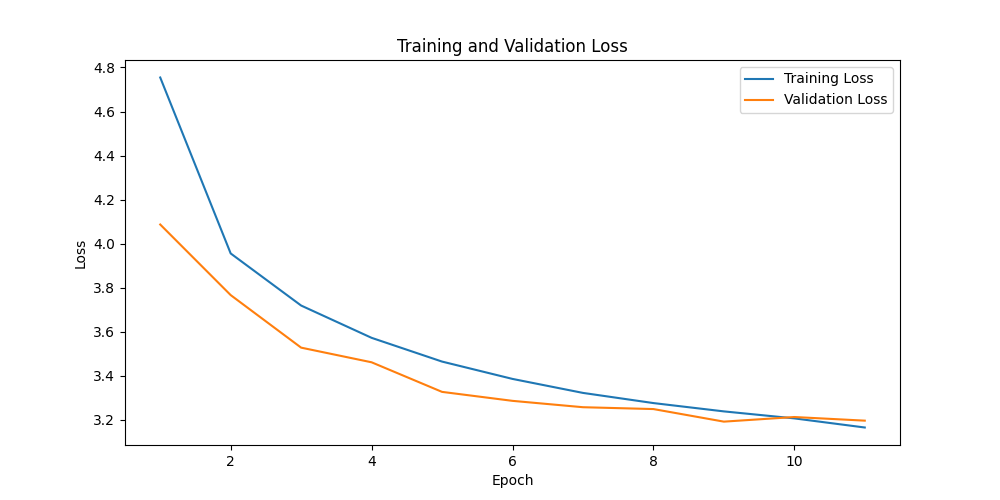
\includegraphics[width=1\textwidth]{Image/loss_plot.png}
    \caption{Sự biến thiên của giá trị loss trên tập huấn luyện và validation qua các epoch}
    \label{fig:loss}
\end{figure}

Nhìn vào đồ thị, có thể thấy giá trị loss giảm đều qua các epoch, cho thấy mô hình học tốt và không bị overfitting. Đến cuối quá trình huấn luyện, loss trên tập validation tiệm cận loss trên tập huấn luyện, chứng tỏ mô hình tổng quát hóa tốt trên dữ liệu đáng kinh ngạc.

\subsection*{5. Quy trình xử lí}
\addcontentsline{toc}{subsection}{Quy trình xử lí}

Quy trình tạo chú thích ảnh tự động bao gồm các bước chính sau đây:
\begin{itemize}
    \item \textbf{Bước 1: } Tiền xử lý dữ liệu: Ảnh và chú thích được chuẩn hóa trước khi đưa vào mô hình. Ảnh được resize, chuyển sang định dạng phù hợp và chuẩn hóa bằng hàm tiền xử lý của CLIP. Các chú thích được tách từ, chuyển về chữ thường, loại bỏ ký tự đặc biệt và mã hóa thành chuỗi số nguyên dựa trên từ điển.
    \item \textbf{Bước 2: } Trích xuất đặc trưng ảnh: Ảnh sau khi tiền xử lý được đưa vào mô hình CLIP để trích xuất vector đặc trưng, đại diện cho nội dung hình ảnh trong không gian đa chiều.
    \item \textbf{Bước 3: } Sinh chú thích: Đặc trưng ảnh từ CLIP được sử dụng làm đầu vào cho mạng LSTM nhiều lớp có tích hợp Attention. Mạng LSTM sẽ lần lượt sinh ra từng từ trong câu chú thích, với sự hỗ trợ của Attention để tập trung vào các đặc trưng quan trọng của ảnh tại mỗi bước sinh từ.
    \item \textbf{Bước 4: } Tối ưu hóa và đánh giá: Quá trình huấn luyện sử dụng hàm mất mát Cross-Entropy để tối ưu hóa mô hình. Sau khi huấn luyện, mô hình được đánh giá bằng các chỉ số BLEU trên tập kiểm tra để đo lường chất lượng chú thích sinh ra so với chú thích tham chiếu.
    \item \textbf{Bước 5: } Sinh chú thích cho ảnh mới: Khi có ảnh mới, hệ thống sẽ thực hiện các bước tiền xử lý, trích xuất đặc trưng, và sử dụng mô hình đã huấn luyện để sinh ra câu chú thích tự động cho ảnh đó.
\end{itemize}

\begin{figure}[H]
    \centering
    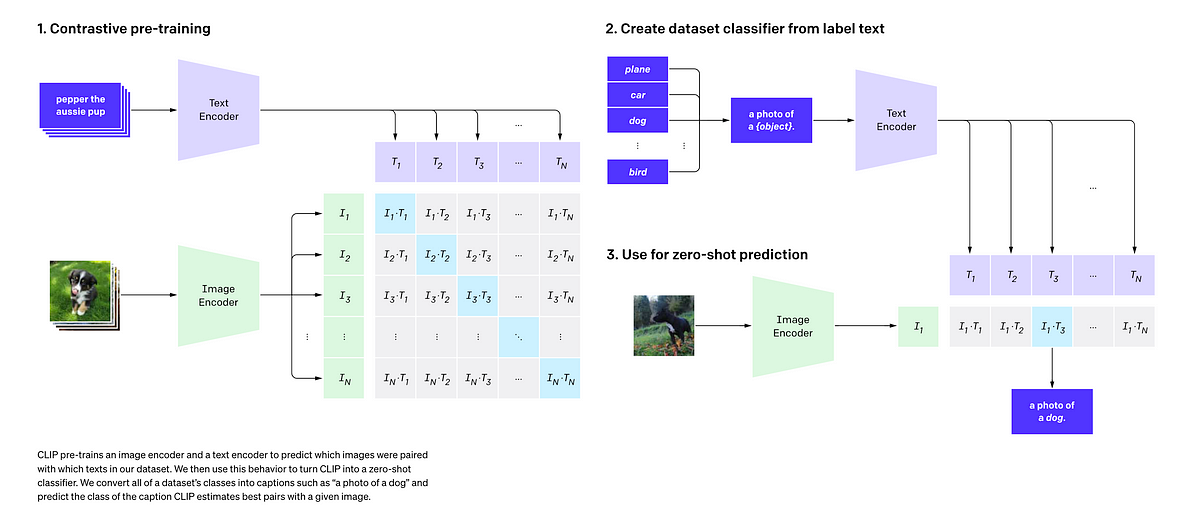
\includegraphics[width=1\textwidth]{Image/imagecaptioning.png}
    \caption{Quy trình sinh chú thích ảnh ảnh}
    \label{fig:loss}
\end{figure}

\subsection*{6. Kết quả}
\addcontentsline{toc}{subsection}{Kết quả}

Trong phần này, nhóm em trình bày kết quả thực nghiệm của mô hình kết hợp CLIP và LSTM trong bài toán tạo chú thích ảnh. Mô hình được đánh giá dựa trên quá trình huấn luyện, các chú thích ảnh được tạo ra, cũng như chỉ số BLEU thể hiện độ chính xác giữa mô tả sinh ra và mô tả gốc.

\subsubsection*{6.1 Quá trình huấn luyện}
\addcontentsline{toc}{subsubsection}{Quá trình huấn luyện}

Quá trình huấn luyện diễn ra trong 15 epoch, tuy nhiên mô hình đã kích hoạt cơ chế dừng sớm (early stopping) tại epoch thứ 11 do không có cải thiện về độ lỗi trên tập validation trong 2 epoch liên tiếp. Trong suốt quá trình huấn luyện, ta nhận thấy rằng loss của cả tập huấn luyện và tập validation đều giảm đều đặn, cho thấy mô hình học tốt và tránh được hiện tượng quá khớp (overfitting). Mô hình tốt nhất đạt được khi validation loss là 3.1911 tại epoch thứ 9.

\begin{figure}[H]
    \centering
    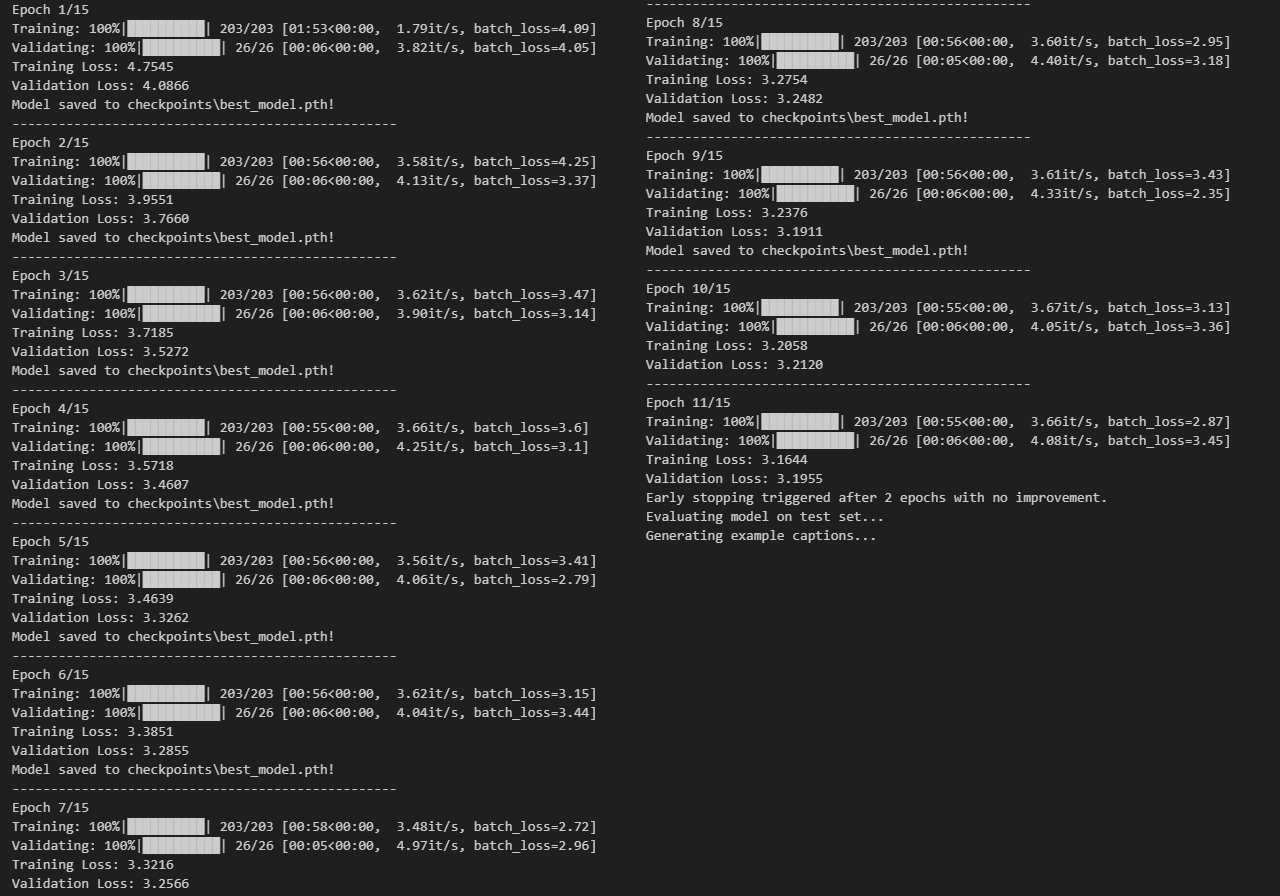
\includegraphics[width=1\textwidth]{Image/result.png}
    \caption{Kết quả huấn luyện mô hình}
    \label{fig:loss}
\end{figure}

\subsubsection*{6.2 Kết quả tạo chú thích ảnh}
\addcontentsline{toc}{subsubsection}{Kết quả tạo chú thích ảnh}

\begin{figure}[H]
    \centering
    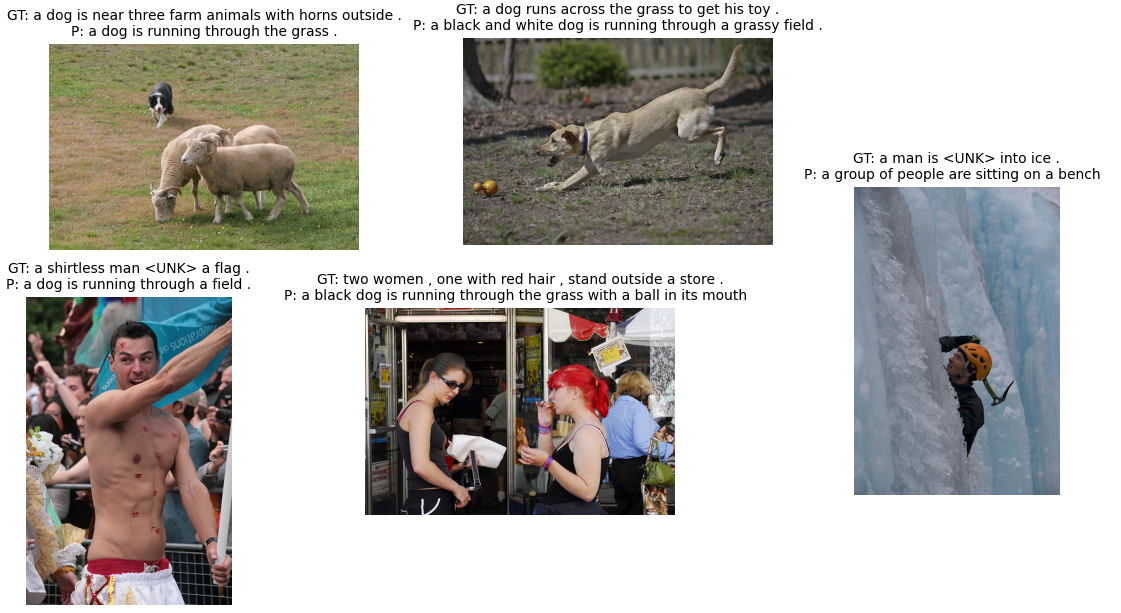
\includegraphics[width=1\textwidth]{Image/result2.png}
    \caption{Kết quả tạo chú thích ảnh}
    \label{fig:loss}
\end{figure}

Sau khi huấn luyện, mô hình được đánh giá trên tập kiểm tra bằng cách so sánh câu mô tả sinh ra (P - Prediction) với câu mô tả gốc (GT - Ground Truth). Tuy nhiên, kết quả cho thấy mô hình vẫn gặp nhiều khó khăn khi tạo ra mô tả chính xác cho ảnh. Nhiều ảnh được mô hình gán chú thích lặp lại hoặc không phù hợp với nội dung thật của ảnh. Ví dụ:
\begin{itemize}
    \item Ảnh một người đàn ông cầm cờ được mô tả sai thành “a dog is running through a field”.
    \item Ảnh hai người phụ nữ đứng trước cửa hàng bị mô hình mô tả thành “a black dog is running through the grass with a ball in its mouth”.
\end{itemize}

Điều này cho thấy mô hình có xu hướng bị hội tụ về các mô tả phổ biến trong dữ liệu huấn luyện, thay vì sinh ra câu mô tả cụ thể theo nội dung ảnh.

\subsubsection*{6.3 Đánh giá mô hình}
\addcontentsline{toc}{subsubsection}{Đánh giá mô hình}

Chỉ số BLEU được sử dụng để đánh giá định lượng chất lượng mô tả ảnh. Kết quả cho thấy các chỉ số BLEU đều ở mức thấp, đặc biệt là BLEU-4 chỉ đạt 0.0201, cho thấy khoảng cách đáng kể giữa câu mô tả mô hình tạo ra và câu mô tả gốc. Cụ thể:
\begin{table}[H]
\centering
\begin{tabular}{|c|c|}
\hline
\textbf{Chỉ số} & \textbf{Giá trị} \\
\hline
BLEU-1 & 0.2706 \\
BLEU-2 & 0.0850 \\
BLEU-3 & 0.0382 \\
BLEU-4 & 0.0201 \\
\hline
\end{tabular}
\caption{Kết quả đánh giá mô hình theo các chỉ số BLEU}
\label{tab:bleu_scores}
\end{table}

\subsubsection*{6.4 Nhận xét}
\addcontentsline{toc}{subsubsection}{Nhận xét}

Mặc dù mô hình kết hợp CLIP và LSTM có khả năng học và giảm lỗi trong quá trình huấn luyện, nhưng chất lượng mô tả đầu ra chưa cao. Chúng ta có thể lý giải lý do vì sao:
\begin{itemize}
    \item Mô hình LSTM đơn giản có thể chưa đủ mạnh để học được các đặc trưng phức tạp của ảnh.
    \item Dữ liệu huấn luyện chưa đủ phong phú, dẫn đến hiện tượng mô hình tạo ra mô tả thiên về các câu phổ biến.
    \item Việc mã hóa thông tin hình ảnh bằng CLIP cần được khai thác hiệu quả hơn hoặc kết hợp thêm kiến trúc sinh mạnh mẽ hơn (ví dụ như Transformer).
\end{itemize}

\subsection*{7. Hạn chế và hướng phát triển}
\addcontentsline{toc}{subsection}{Hạn chế và hướng phát triển}

Tuy mô hình đã hoạt động hiệu quả trong một số trường hợp, đặc biệt là với các ảnh có ngữ cảnh rõ ràng, tuy nhiên cũng còn tồn tại những điểm cần cải thiện để nâng cao độ chính xác và sự phù hợp của mô tả ảnh. Một số vấn đề tiêu biểu có thể kể đến như sau:

\begin{itemize}
    \item \textbf{Thứ nhất: } Mô hình có xu hướng tạo ra các mô tả chung chung, lặp lại hoặc không đúng với nội dung ảnh cụ thể. Ví dụ, nhiều ảnh khác nhau được gán cùng một mô tả như “a dog is running through the grass”, mặc dù trong ảnh không hề có chó hoặc hoạt động tương ứng. Điều này cho thấy mô hình bị ảnh hưởng bởi sự thiên lệch dữ liệu và học theo các mô tả phổ biến thay vì chú thích đúng nội dung.
    \item \textbf{Thứ hai: } Mô hình gặp khó khăn trong việc sinh mô tả cho các ảnh có bố cục phức tạp, nhiều đối tượng, hoặc các chi tiết không phổ biến trong tập huấn luyện. Trong các trường hợp này, câu mô tả thường không đề cập đúng tới hành động, vật thể chính, hoặc thậm chí mô tả sai hoàn toàn.
    \item \textbf{Thứ ba: } Chỉ số BLEU ở các cấp độ (từ BLEU-1 đến BLEU-4) đều đạt giá trị thấp, đặc biệt BLEU-4 chỉ ở mức 0.0201, cho thấy mô hình chưa học được tốt mối quan hệ giữa đặc trưng ảnh và ngôn ngữ mô tả. Điều này phần lớn do giới hạn của mô hình LSTM trong việc học chuỗi dài và khả năng sinh ngữ cảnh chính xác.
    \item \textbf{Thứ tư: } Beam search với kích thước cố định không phải lúc nào cũng sinh ra chú thích tối ưu. Đôi khi các chú thích có điểm số cao nhất lại thiếu tự nhiên hoặc quá đơn giản so với nội dung phức tạp của ảnh. Hiện tượng này xuất hiện khi mô hình ưu tiên các chuỗi từ an toàn nhưng ít thông tin.
\end{itemize}

Nhóm em đã nghiên cứu và đưa ra kết luận rằng các vấn đề trên xảy ra do hai nguyên nhân chính: hạn chế về kích thước và đa dạng của tập dữ liệu huấn luyện, cùng với cấu trúc đơn giản của mô hình so với độ phức tạp của bài toán tạo chú thích ảnh.

Về hướng phát triển trong tương lai, nhóm em dự định sẽ:
\begin{itemize}
    \item \textbf{Hướng thứ nhất: } Tích hợp cơ chế Attention tinh vi hơn để mô hình có thể tập trung vào các vùng quan trọng khác nhau của ảnh khi sinh từng từ trong caption. Cụ thể, có thể áp dụng Self-Attention hoặc Multi-Head Attention để nắm bắt tốt hơn mối quan hệ không gian giữa các đối tượng trong ảnh.
    \item \textbf{Hướng thứ hai: } Sử dụng bộ dữ liệu lớn và đa dạng hơn như COCO hoặc Conceptual Captions để mở rộng khả năng nhận biết đối tượng và ngôn ngữ của mô hình. Việc kết hợp nhiều bộ dữ liệu khác nhau cũng có thể giúp mô hình khái quát hóa tốt hơn.
    \item \textbf{Hướng thứ ba: } Thay thế LSTM bằng các kiến trúc hiện đại hơn như Transformer, kết hợp với pre-trained language models như GPT để cải thiện chất lượng ngôn ngữ của các caption được tạo ra. Điều này sẽ giúp tạo ra các chú thích tự nhiên và đa dạng hơn về mặt ngôn ngữ.
\end{itemize}

Do hướng tài nguyên phần cứng và thời gian có hạn, ba hướng nghiên cứu trên nhóm em chưa thể triển khai đầy đủ ở thời điểm hiện tại. Tuy nhiên, các thử nghiệm ban đầu với việc tăng cường cơ chế Attention đã cho thấy kết quả khả quan, hứa hẹn cải thiện đáng kể chất lượng chú thích trong tương lai.
\end{document}

